\documentclass[12pt]{amsart}
\usepackage[symbol]{footmisc}
\usepackage{float}

\usepackage{style_template}
\renewcommand*{\thefootnote}{\fnsymbol{footnote}}

% \newtheorem{theorem}{Theorem}
% \newtheorem{definition}{Definition}

\title{Fair Decision Making}
\author{David Yang$^{\dagger}$, Selena She$^{\dagger}$, Amy Feng$^{\dagger}$, Alexander Goslin$^{\dagger}$}
\date{Summer 2023}

\begin{document}

\maketitle

\begin{center}
    Note: $\dagger$ denotes equal contribution.
\end{center}

\section{General Background Reading}
\subsection{\href{https://arxiv.org/abs/1406.2661}{Generative Adversarial Networks}}

\begin{definition}[Generator]
A \textbf{generator} is a neural network that learns to generate realistic samples by transforming random noise into data samples that resemble the training data.
\end{definition}

\begin{definition}[Discriminator]
A \textbf{discriminator} is a neural network that aims to distinguish between real and fake examples.
\end{definition}

More formally, a generative model captures the data distribution and a discriminative model estimates the probability that a sample came from the training data rather than G. "The generative model can be thought of as analogous to a team of counterfeiters, trying to produce fake currency and use it without detection, while the discriminative model is analogous to the police, trying to detect the counterfeit currency."

\begin{definition}[Adversarial Nets]
\textbf{Adversarial nets} refer to the specific case where the generative model generates samples by passing random noise through a multilayer perceptron, and the discriminative model is also a multilayer perceptron. 
\end{definition}

\vspace{0.5cm}

\subsection{\href{https://arxiv.org/abs/2006.11239}{Denoising Diffusion Probabilistic Model} / \href{https://arxiv.org/abs/2010.02502}{Denoising Diffusion Implicit Model}}

\textit{Other Relevant Resource(s):} \href{https://strikingloo.github.io/wiki/ddim#:~:text=Properties%20of%20DDIM%20vs%20DDPM,have%20similar%20high%2Dlevel%20features}{DDIM vs DDPM Article}

\begin{definition}[Diffusion Model]
A \textbf{diffusion (probabilistic) model} is a parameterized Markov chain trained using variational inference to produce samples matching the data after finite time.  
\end{definition}

DDPMs are types of generative models that use probabilistic processes to transform the data from a simple distribution to a more complex target distribution. It iteratively refines the initial random distribution, where in each step it removes the noise from the data and eventually ends up creating a realistic sample of data. In comparison to Generative Adversarial Nets (GANs), GANs may suffer from \textbf{real mode collapse} in which the generator produces just a small variety of data that is not as diverse as real-world data. On the other hand, diffusion models will not have this problem but may take longer/tend to be more computationally expensive. \\

\begin{definition}[DDIM]
A \textbf{Denoising diffusion implicit model (DDIM)} is a more efficient class of iterative implicit probabilistic models with the same training procedure as DDPMs.
\end{definition}

The generative process of a DDPM is defined as the ``reverse of a Markovian diffusion process," which approximates the reverse of the forward diffusion process (from data to noise) and is much slower than a GAN, which typically requires only one pass through a network. On the other hand, a DDIM allows for much faster sampling while keeping an equivalent training objective, so that generative models using this architecture are competitive to GANs at the same model size/sample quality." This is done by ``estimating the addition of multiple Markov chain jumps by estimating the sum of Gaussian Markov jumps as Gaussian." This generalizes the Markovian forward diffusion process of DDPMs to a non-Markovian one. \\

One of the key differences between the DDIM and DDPMs is the ``\textbf{consistency}" property (present in DDIMs but not DDPMs): if we start with the same initial latent variable and generate several samples with Markov chains of various lengths, these samples would have similar high-level features. The consistency of DDIMs allow for meaningful image interpolation.

\subsection{\href{https://arxiv.org/pdf/2211.05617.pdf}{Debiasing Methods for Fairer Neural Models in Vision and Language Research: A Survey}}

\begin{definition}[Fairness]
\textbf{Fairness} refers to the ``absence of any prejudice or favoritism toward an individual or a group based on their inherent or acquired characteristics."
\end{definition}

\begin{definition}[Bias]
\textbf{Bias} is any unintended behavior resulting from correlation-based processing that ignores further context not explicit in the data.
\end{definition}

Different types of bias include \textbf{inductive bias} (unavoidable bias inherent to the learning task), \textbf{data bias} (bias of representation/sampling/measurement of data towards a group of subjects) and \textbf{intersectional bias} (when an underprivileged group defined by a combination of sensitive attribute and  dynamics of individuals are considerably distinct than when considering one sensitive attribute at a time). \\

We can test the embedding of a given prompt for bias to measure bias in language models. Metrics to measure bias include \href{https://arxiv.org/pdf/1607.06520.pdf}{\textbf{Direct Bias (DB)}}, where we measure the bias as a projection onto a gender subspace, the \href{https://purehost.bath.ac.uk/ws/portalfiles/portal/168480066/CaliskanEtAl_authors_full.pdf}{\textbf{Word Embedding Association Test (WEAT)}} which measures bias through permutation of two sets of target words and two sets of attribute words (e.g. engineers/nurses and male/female). The \href{https://arxiv.org/pdf/1903.10561.pdf}{\textbf{Sentence Embedding Association Test (SEAT)}} is similar to WEAT but works for contextualized word embeddings. \\

\begin{definition}[Existing Debiasing Categorization]
Debiasing approaches are typically divided into three categories: \textbf{preprocessing} (transform the data so that the underlying
discrimination is removed), \textbf{inprocessing} (modify and change state-of-the-art learning
algorithms in order to remove discrimination during the model training process), and \textbf{postprocessing} (performed after training).
\end{definition}

\textit{Note: we anticipate that our approaches will be of the postprocessing type.} \\

The survey paper introduces a new taxonomy to categorize debiasing methods: 

\begin{definition}[New Taxonomy for Debiasing Methods]
A \textbf{distributional} strategy modifies the dataset prior to training. \\

An \textbf{inferential} strategy that addresses the problem of fairness based on the model outputs, i.e. that discover and remove social biases without requiring further weight optimization or dataset manipulation
\end{definition}

There is also a distinction between methods that focus on optimization via training into two categories:
\begin{definition}[1-Step and 2-Step Training]
\textbf{One-step-training} includes fair models generated for a particular task via a single optimization procedure, whereas \textbf{Two-step-training} includes models where a new training phase must be performed to fix an existing biased model.
\end{definition}

There a few methods to debias one-step-training models:
\begin{definition}[Groups of One-Step-Learning Debiasing Methods]
\textbf{Adversarial} methods use adversarial examples to teach the model not to resort to undesired biases. \\

\textbf{Causal} methods leverage knowledge on causal-effect between protected attributes and outcomes to fix model unfairness (e.g. create new examples during training/generate ``counterfactual samples"). \\

\textbf{Disentanglement} methods break down features in latent space to manipulate information independently. \\

\textbf{Optimization} methods include loss function adaptions, the addition of regularization terms, and other modifications for improving weight optimization. 
\end{definition}

\begin{discussion*}
Of the four one-step-learning debiasing methods discussed above, we anticipate looking at \textbf{Adversarial} methods and \textbf{Disentanglement} methods. \\

An adversarial approach may work similarly to in the following \href{https://arxiv.org/pdf/2203.11933.pdf}{Adversarial Learning Debiasing Method} paper, and a related-to-disentanglement approach is discussed in this \href{https://arxiv.org/pdf/2302.00070.pdf}{Debiasing VLMs via Biased Prompts} paper (that being said, this approach may be better categorized as \textbf{Vector-Space Manipulation}, which is described later).
\end{discussion*}

Inferential models are distinct from distributional models since they intervene during \textit{inference time} (post-training) to make models fairer.

\begin{definition}[Inferential Models]
\textbf{Prompting} prepends or alters the model input with specific triggers that stimulate a bias-free result. \\

\textbf{Vector-Space Manipulation} manipulates the embedding space to remove undesired biases.
\end{definition}

\begin{discussion*}
We've already seen these two approaches (prompting and vector-space manipulation) in other papers; specifically, the Fair Diffusion (\ref{fairdiffusion}) paper is an example of a prompting approach whereas the Debiasing VLMs paper (\ref{embedding}) paper takes a vector-space manipulation approach.
\end{discussion*}


\newpage

\section{Focused Readings}
\subsection{\href{https://arxiv.org/abs/2302.10893}{Fair Diffusion: Instructing Text-to-Image Generation Models on Fairness}}\label{fairdiffusion}

\begin{approach*}
\textbf{Fair Diffusion} is a strategy that attenuates biases after the deployment of generative text-to-image models. It shifts a bias, based on human instructions, in any direction yielding arbitrary proportions (e.g. identity groups), by instructing a pre-trained model on fairness during the deployment stage.
\end{approach*}

Fair Diffusion is evaluated with Hugging Face's \href{https://huggingface.co/docs/diffusers/api/pipelines/semantic_stable_diffusion}{Semantic Guidance} pipeline, which allows for changes to image generation to be more easily controlled (and thus enable it to stay closer to the original image composition). To classify the gender of the generated images, they use the pre-trained \href{https://arxiv.org/pdf/1908.04913.pdf}{FairFace classifier}.\\

For example, consider the following pairs of images, generated with stable diffusion and fair diffusion: 

\setlength\intextsep{0pt}{
\begin{figure}[H]
    \centering
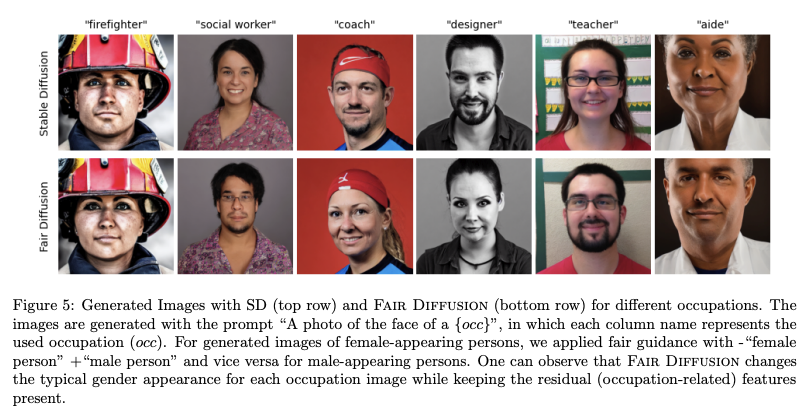
\includegraphics[scale = 0.45]{FairDiffusion_BeforeAndAfter.png}\label{fig:fairdiffusion_comparison}
\end{figure}}

We notice that, despite correcting for the protected attribute of gender, the remainder of the generated images' characteristics stay the same. 
\begin{figure}[H]
    \centering
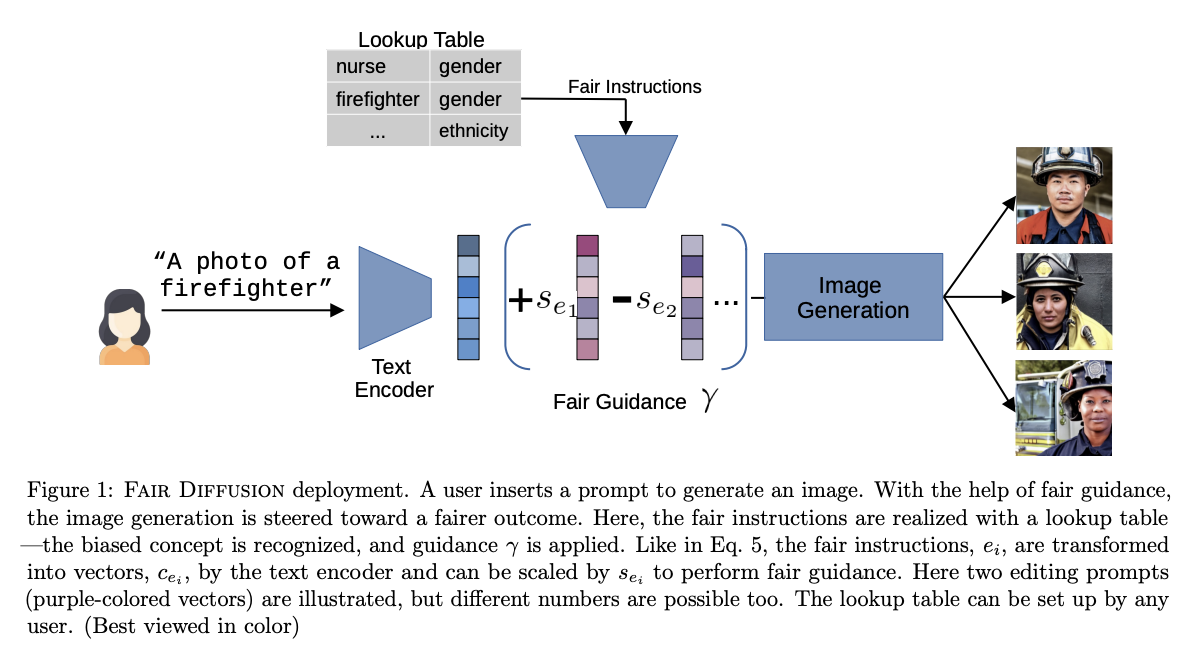
\includegraphics[scale = 0.65]{FairDiffusion_Method.png}
    \label{fig:fairdiffusion_method}
\end{figure}

As discussed in the paper, fair diffusion works at the following high-level manner: the generated image $x$ satisfies
\[ x = \eta(p, \gamma(e, s_e)).\]

More specifically, $\eta$ is a function of the text input prompt $p$ (e.g., "A photo of a firefighter") with "fair guidance"
, $\gamma$, given during the generation. In turn, $\gamma$ depends on additional textual descriptions of attribute expressions $e_i$, scaled by $s_{e_i}$ with guidance direction. As a result, the image generation is guided towards the input prompt p
and fairness instructions $e_i$ simultaneously. \\

To realize the different expressions of an attribute with Fair
Diffusion, the authors control the guidance direction by randomly sampling from a desired probability distribution P. That
means each $e_i$ is either increased or decreased depending on the expression that should be promoted/suppressed. \\

The above figure displays a binary case  where concept $e_1$ is promoted (+) and $e_2$ is suppressed (-) during the image
generation -- their direction can be changed based on P. The purpose of the \textbf{lookup table} is to identify prompts requiring fair guidance and to align the output with the users’ fairness notions.


\noindent\rule{\textwidth}{1pt}

\vspace{0.5cm}
Another area this paper investigates is ``bias inspection" in the components of the well-known text-to-image generation model \href{https://huggingface.co/blog/stable_diffusion}{Stable Diffusion}. Stable Diffusion relies on the large-scale image dataset LAION-5B and the pre-trained text encoder model \href{https://huggingface.co/docs/transformers/model_doc/clip#transformers.CLIPTextModel}{CLIP}. \\

In the subset of the image dataset LAION-5B that the paper uses, they found that the ``Science" and ``Engineering" subsets have lower rates of female-appearing persons (around 0.35 and 0.2, respectively), while ``Arts" and ``Caregiving" (around 0.55 and 0.75, respectively) have higher rates of female-appearing persons, reflecting stereotypical gender occupation biases. \\

Similar biases are revealed after the authors use the iEAT Bias Test for CLIP: \\

\begin{figure}[H]
    \centering
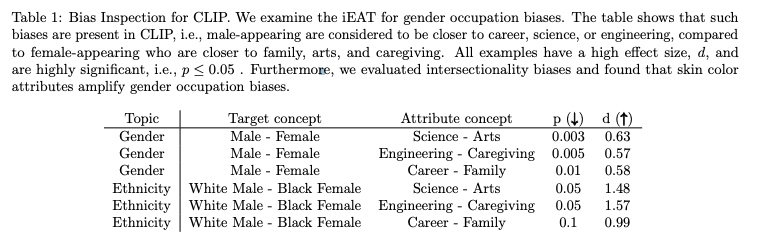
\includegraphics[scale = 0.6]{FairDiffusion_CLIP_Bias.png}
    \label{fig:clip_bias}
\end{figure}
In fact, bias amplification occurs when the association is modified by ethnic attributes (males as European and females as African-American). \\

To summarize the results, the authors ``found biases and unfairness in each component of the SD pipeline: in the LAION-5B dataset, in the CLIP encoder, and in the generated images. At the same time, the biases are not simply mirrored between LAION-5B and SD’s outcome and do not show a clear tendency."

\begin{discussion*}
The prompts in this paper are all of the format ``give me a photo of the face of a [ ]." \\

A specific ambiguous case mentioned is the ``face of a dishwasher” (which gives a photo of a dishwasher rather than someone washing the dishes). Consequently, can the given prompt be modified to ``the face of a person washing dishes" (or other similar formats), and how might these shifts affect the paper's results?
\end{discussion*}

\begin{extension*}
Implicit associations are not accounted for (this paper requires a lookup table mapping pre-defined occupations to protected groups). However, a prompt such as “a photo of a hospital” may generate images where doctors are predominately male. \\

\noindent \textbf{Can we extend or modify the existing work to support biases implied from text prompts?} 
\end{extension*}

\newpage

\subsection{\href{https://arxiv.org/pdf/2302.00070.pdf}{Debiasing Vision-Language Models via Biased Prompts}}\label{embedding}

\begin{approach*}
Many approaches for debiasing Vision-Language Models require training or fine-tuning models using resampled datasets, or modified objectives, which can be computationally expensive. The paper proposes a general approach for "self-debiasing foundation vision-language models by projecting out biased directions in the text embedding." \\

This approach creates a projection matrix (where each row is an attribute) that projects out biased directions. To address possible unstabilities caused by prompts defining the biased directions, they use ``positive pairs" (pairs of prompts that are expected to have the same semantic meaning after projection) to calibrate the projection matrix. Their overall approach does not require training, data, or labels, so it is computationally efficient.
\end{approach*}

The bias of a classifier will be quantified by computing the cosine similarity between its weights and the corresponding spurious feature. We expect rows of classifier weights to have similar cosine similarities to pairs of embeddings: for example, the embedding of ``a photo of a doctor" should be similar to ``a photo of a male doctor" and ``a photo of a female doctor."

\begin{approach*}
To evaluate generative models, the paper uses the CLIP classifier to predict the sensitive attributes and human evaluation to corroborate these results. \\

They mention that as an alternative, the FairFace classifier could be used. However, they note that the ``domain shift between the FairFace dataset and the generated images significantly impaired performance" and thus used the CLIP classifier.
\end{approach*}

\begin{discussion*}
This paper mentions that FairFace dataset and the generated images significantly impacts the bias/general performance (so they used CLIP) but the Diffusion Paper (\ref{fairdiffusion}) used FairFace as the final classifier. \\ 

We will need to be cognizant of our choice, specifically how the classifiers work on our generated images.
\end{discussion*}

\newpage

\subsection{\href{https://arxiv.org/pdf/2103.00020.pdf}{Learning Transferable Visual Models from Natural Language Supervision (CLIP)}}

\begin{approach*} \textbf{CLIP} (Contrastive Language-Image Pre-training), is an efficient method of learning from natural language supervision. \\

Given a batch of $N$ (image, text) pairs, CLIP is trained to predict which of the $N \times N$ possible (image, text) pairings across a batch occurred. They do this by jointly training an image encoder and text encoder to maximize the cosine similarity of the image and text embeddings of the N real pairs in the batch.
\end{approach*}
\end{document}
